% Options for packages loaded elsewhere
\PassOptionsToPackage{unicode}{hyperref}
\PassOptionsToPackage{hyphens}{url}
\PassOptionsToPackage{dvipsnames,svgnames,x11names}{xcolor}
%
\documentclass[
  letterpaper,
  DIV=11,
  numbers=noendperiod]{scrreprt}

\usepackage{amsmath,amssymb}
\usepackage{iftex}
\ifPDFTeX
  \usepackage[T1]{fontenc}
  \usepackage[utf8]{inputenc}
  \usepackage{textcomp} % provide euro and other symbols
\else % if luatex or xetex
  \usepackage{unicode-math}
  \defaultfontfeatures{Scale=MatchLowercase}
  \defaultfontfeatures[\rmfamily]{Ligatures=TeX,Scale=1}
\fi
\usepackage{lmodern}
\ifPDFTeX\else  
    % xetex/luatex font selection
\fi
% Use upquote if available, for straight quotes in verbatim environments
\IfFileExists{upquote.sty}{\usepackage{upquote}}{}
\IfFileExists{microtype.sty}{% use microtype if available
  \usepackage[]{microtype}
  \UseMicrotypeSet[protrusion]{basicmath} % disable protrusion for tt fonts
}{}
\makeatletter
\@ifundefined{KOMAClassName}{% if non-KOMA class
  \IfFileExists{parskip.sty}{%
    \usepackage{parskip}
  }{% else
    \setlength{\parindent}{0pt}
    \setlength{\parskip}{6pt plus 2pt minus 1pt}}
}{% if KOMA class
  \KOMAoptions{parskip=half}}
\makeatother
\usepackage{xcolor}
\setlength{\emergencystretch}{3em} % prevent overfull lines
\setcounter{secnumdepth}{5}
% Make \paragraph and \subparagraph free-standing
\makeatletter
\ifx\paragraph\undefined\else
  \let\oldparagraph\paragraph
  \renewcommand{\paragraph}{
    \@ifstar
      \xxxParagraphStar
      \xxxParagraphNoStar
  }
  \newcommand{\xxxParagraphStar}[1]{\oldparagraph*{#1}\mbox{}}
  \newcommand{\xxxParagraphNoStar}[1]{\oldparagraph{#1}\mbox{}}
\fi
\ifx\subparagraph\undefined\else
  \let\oldsubparagraph\subparagraph
  \renewcommand{\subparagraph}{
    \@ifstar
      \xxxSubParagraphStar
      \xxxSubParagraphNoStar
  }
  \newcommand{\xxxSubParagraphStar}[1]{\oldsubparagraph*{#1}\mbox{}}
  \newcommand{\xxxSubParagraphNoStar}[1]{\oldsubparagraph{#1}\mbox{}}
\fi
\makeatother


\providecommand{\tightlist}{%
  \setlength{\itemsep}{0pt}\setlength{\parskip}{0pt}}\usepackage{longtable,booktabs,array}
\usepackage{calc} % for calculating minipage widths
% Correct order of tables after \paragraph or \subparagraph
\usepackage{etoolbox}
\makeatletter
\patchcmd\longtable{\par}{\if@noskipsec\mbox{}\fi\par}{}{}
\makeatother
% Allow footnotes in longtable head/foot
\IfFileExists{footnotehyper.sty}{\usepackage{footnotehyper}}{\usepackage{footnote}}
\makesavenoteenv{longtable}
\usepackage{graphicx}
\makeatletter
\newsavebox\pandoc@box
\newcommand*\pandocbounded[1]{% scales image to fit in text height/width
  \sbox\pandoc@box{#1}%
  \Gscale@div\@tempa{\textheight}{\dimexpr\ht\pandoc@box+\dp\pandoc@box\relax}%
  \Gscale@div\@tempb{\linewidth}{\wd\pandoc@box}%
  \ifdim\@tempb\p@<\@tempa\p@\let\@tempa\@tempb\fi% select the smaller of both
  \ifdim\@tempa\p@<\p@\scalebox{\@tempa}{\usebox\pandoc@box}%
  \else\usebox{\pandoc@box}%
  \fi%
}
% Set default figure placement to htbp
\def\fps@figure{htbp}
\makeatother
% definitions for citeproc citations
\NewDocumentCommand\citeproctext{}{}
\NewDocumentCommand\citeproc{mm}{%
  \begingroup\def\citeproctext{#2}\cite{#1}\endgroup}
\makeatletter
 % allow citations to break across lines
 \let\@cite@ofmt\@firstofone
 % avoid brackets around text for \cite:
 \def\@biblabel#1{}
 \def\@cite#1#2{{#1\if@tempswa , #2\fi}}
\makeatother
\newlength{\cslhangindent}
\setlength{\cslhangindent}{1.5em}
\newlength{\csllabelwidth}
\setlength{\csllabelwidth}{3em}
\newenvironment{CSLReferences}[2] % #1 hanging-indent, #2 entry-spacing
 {\begin{list}{}{%
  \setlength{\itemindent}{0pt}
  \setlength{\leftmargin}{0pt}
  \setlength{\parsep}{0pt}
  % turn on hanging indent if param 1 is 1
  \ifodd #1
   \setlength{\leftmargin}{\cslhangindent}
   \setlength{\itemindent}{-1\cslhangindent}
  \fi
  % set entry spacing
  \setlength{\itemsep}{#2\baselineskip}}}
 {\end{list}}
\usepackage{calc}
\newcommand{\CSLBlock}[1]{\hfill\break\parbox[t]{\linewidth}{\strut\ignorespaces#1\strut}}
\newcommand{\CSLLeftMargin}[1]{\parbox[t]{\csllabelwidth}{\strut#1\strut}}
\newcommand{\CSLRightInline}[1]{\parbox[t]{\linewidth - \csllabelwidth}{\strut#1\strut}}
\newcommand{\CSLIndent}[1]{\hspace{\cslhangindent}#1}

\KOMAoption{captions}{tableheading}
\makeatletter
\@ifpackageloaded{bookmark}{}{\usepackage{bookmark}}
\makeatother
\makeatletter
\@ifpackageloaded{caption}{}{\usepackage{caption}}
\AtBeginDocument{%
\ifdefined\contentsname
  \renewcommand*\contentsname{Table of contents}
\else
  \newcommand\contentsname{Table of contents}
\fi
\ifdefined\listfigurename
  \renewcommand*\listfigurename{List of Figures}
\else
  \newcommand\listfigurename{List of Figures}
\fi
\ifdefined\listtablename
  \renewcommand*\listtablename{List of Tables}
\else
  \newcommand\listtablename{List of Tables}
\fi
\ifdefined\figurename
  \renewcommand*\figurename{Figure}
\else
  \newcommand\figurename{Figure}
\fi
\ifdefined\tablename
  \renewcommand*\tablename{Table}
\else
  \newcommand\tablename{Table}
\fi
}
\@ifpackageloaded{float}{}{\usepackage{float}}
\floatstyle{ruled}
\@ifundefined{c@chapter}{\newfloat{codelisting}{h}{lop}}{\newfloat{codelisting}{h}{lop}[chapter]}
\floatname{codelisting}{Listing}
\newcommand*\listoflistings{\listof{codelisting}{List of Listings}}
\makeatother
\makeatletter
\makeatother
\makeatletter
\@ifpackageloaded{caption}{}{\usepackage{caption}}
\@ifpackageloaded{subcaption}{}{\usepackage{subcaption}}
\makeatother

\usepackage{bookmark}

\IfFileExists{xurl.sty}{\usepackage{xurl}}{} % add URL line breaks if available
\urlstyle{same} % disable monospaced font for URLs
\hypersetup{
  pdftitle={Evaluation of Not Safe For Work},
  pdfauthor={Jia Yee Wong},
  colorlinks=true,
  linkcolor={blue},
  filecolor={Maroon},
  citecolor={Blue},
  urlcolor={Blue},
  pdfcreator={LaTeX via pandoc}}


\title{Evaluation of Not Safe For Work}
\author{Jia Yee Wong}
\date{}

\begin{document}
\maketitle

\renewcommand*\contentsname{Table of contents}
{
\hypersetup{linkcolor=}
\setcounter{tocdepth}{2}
\tableofcontents
}

\bookmarksetup{startatroot}

\chapter*{Preface}\label{preface}
\addcontentsline{toc}{chapter}{Preface}

\markboth{Preface}{Preface}

You are a data scientist for a mid-sized business, in a small group of
3-4 data scientists. You've been tasked with creating a report
evaluating a scenario for your business. Your colleagues will also be
evaluating the same scenario, and your reports will be used in aggregate
to determine a consensus (or lack thereof) on the company's action. The
reports will also be used to inform downsizing that is rumored to be
coming - you want to ensure your report is better than your peers so
that you aren't as easy to cut.

You may talk to your peers who are assigned the same scenario, but you
do not want to collaborate too closely, lest you both become targets of
the rumored layoffs.

\begin{center}\rule{0.5\linewidth}{0.5pt}\end{center}

I've scaffolded this report for you to make this process easier - as we
talk about different sections of a report in class and read about how to
create similar sections, you will practice by writing the equivalent
section of your report.

The basic steps for this task are as follows:

\begin{itemize}
\item
  Identify the research question from the business question
\item
  Identify data set(s) which are (1) publicly available (you don't have
  a budget to pay for private data) and (2) relevant to your task

  \begin{itemize}
  \tightlist
  \item
    (HW Week 6) Document your data sets in \texttt{draft-data-doc.qmd}
  \end{itemize}
\item
  Conduct a statistical analysis to support your answer to your research
  and business questions

  \begin{itemize}
  \item
    Write a methods section for your business report corresponding to
    your statistical analysis
  \item
    (HW Week 9) Draft of results section of business report with
    relevant graphics/visual aids in \texttt{draft-results.qmd}
  \end{itemize}
\item
  Write your report

  \begin{itemize}
  \item
    (HW Week 10) Draft of Intro/Conclusion sections in
    \texttt{draft-intro-conclusions.qmd}
  \item
    (HW Week 11) Draft of Executive summary section in
    \texttt{draft-exec-summary.qmd}
  \end{itemize}
\item
  Revise your report

  \begin{itemize}
  \item
    (HW Week 12 -- not turned in) Revise your report
  \item
    (HW Week 13) - Rough draft of report due. Create one or more qmd
    files for your report (you can overwrite or delete intro.qmd and
    summary.qmd), include the names of each file (in order) in
    \texttt{\_quarto.yml}. You should use references (edit
    references.bib and use pandoc citations). Make sure your report
    compiles and looks reasonable in both html and pdf.
  \item
    Develop a presentation to go along with your report (Week 13).
    Create slides for your report using quarto.
  \end{itemize}
\item
  Peer revise reports

  \begin{itemize}
  \item
    Peer revise reports
  \item
    (HW Week 14) - Make edits to your report from comments received from
    peer review
  \end{itemize}
\item
  Final report \& presentation due
\end{itemize}

\bookmarksetup{startatroot}

\chapter{Introduction}\label{introduction}

This is a book created from markdown and executable code.

See Knuth (1984) for additional discussion of literate programming.

\bookmarksetup{startatroot}

\chapter{Summary}\label{summary}

In summary, this book has no content whatsoever.

\bookmarksetup{startatroot}

\chapter*{References}\label{references}
\addcontentsline{toc}{chapter}{References}

\markboth{References}{References}

\phantomsection\label{refs}
\begin{CSLReferences}{1}{0}
\bibitem[\citeproctext]{ref-AmazonFinedNearly}
{``Amazon {Is Fined Nearly} \$6 {Million Over Warehouse Work Quotas} -
{The New York Times}.''} n.d. Accessed April 5, 2025.
\url{https://www.nytimes.com/2024/06/18/business/economy/amazon-california-productivity-quota.html}.

\bibitem[\citeproctext]{ref-CensusFatalOccupational}
{``Census of {Fatal Occupational Injuries Summary}, 2023 - 2023 {A01
Results}.''} n.d. Bureau of Labor Statistics. Accessed March 5, 2025.
\url{https://www.bls.gov/news.release/cfoi.nr0.htm}.

\bibitem[\citeproctext]{ref-EmployerReportedWorkplaceInjuries}
{``Employer-{Reported Workplace Injuries} and {Illnesses}, 2023 - 2023
{A01 Results}.''} n.d. Bureau of Labor Statistics. Accessed March 5,
2025. \url{https://www.bls.gov/news.release/osh.nr0.htm}.

\bibitem[\citeproctext]{ref-IIFHome}
{``{IIF Home}.''} n.d. Bureau of Labor Statistics. Accessed March 10,
2025. \url{https://www.bls.gov/iif/}.

\bibitem[\citeproctext]{ref-knuth84}
Knuth, Donald E. 1984. {``Literate Programming.''} \emph{Comput. J.} 27
(2): 97--111. \url{https://doi.org/10.1093/comjnl/27.2.97}.

\bibitem[\citeproctext]{ref-NIOSHWorkerHealth2024}
{``{NIOSH Worker Health Charts}.''} 2024. February 12, 2024.
\url{https://wwwn.cdc.gov/NIOSH-WHC/chart/bls-ii/injury?T=ZS&V=C&D=RANGE&chk_codes=False}.

\bibitem[\citeproctext]{ref-WorkInjuryCosts}
{``Work {Injury Costs}.''} n.d. Injury Facts. Accessed April 5, 2025.
\url{https://injuryfacts.nsc.org/work/costs/work-injury-costs/}.

\end{CSLReferences}

(\textbf{online?})\{CensusFatalOccupational, title = \{Census of
\{\{Fatal Occupational Injuries Summary\}\}, 2023 - 2023 \{\{A01
Results\}\}\}, url = \{https://www.bls.gov/news.release/cfoi.nr0.htm\},
urldate = \{2025-03-05\}, langid = \{english\}, organization = \{Bureau
of Labor Statistics\}, file =
\{/Users/jiayeewong/Zotero/storage/CYAKQ4PJ/cfoi.nr0.html\} \}

(\textbf{online?})\{EmployerReportedWorkplaceInjuries, title =
\{Employer-\{\{Reported Workplace Injuries\}\} and \{\{Illnesses\}\},
2023 - 2023 \{\{A01 Results\}\}\}, url =
\{https://www.bls.gov/news.release/osh.nr0.htm\}, urldate =
\{2025-03-05\}, langid = \{english\}, organization = \{Bureau of Labor
Statistics\}, file =
\{/Users/jiayeewong/Zotero/storage/73EPJTYT/osh.nr0.html\} \}

(\textbf{online?})\{IIFHome, title = \{\{\{IIF Home\}\}\}, url =
\{https://www.bls.gov/iif/\}, urldate = \{2025-03-10\}, langid =
\{english\}, organization = \{Bureau of Labor Statistics\}, file =
\{/Users/jiayeewong/Zotero/storage/I8GRUP7W/iif.html\} \}

(\textbf{online?})\{IIFLatestNumbers, title = \{\{\{IIF Latest
Numbers\}\}\}, url = \{https://www.bls.gov/iif/latest-numbers.htm\},
urldate = \{2025-03-10\}, langid = \{english\}, organization = \{Bureau
of Labor Statistics\}, file =
\{/Users/jiayeewong/Zotero/storage/5FF2NSMM/latest-numbers.html\} \}

(\textbf{online?})\{NIOSHWorkerHealth2024, title = \{\{\{NIOSH Worker
Health Charts\}\}\}, date = \{2024-02-12T11:57:02Z\}, url =
\{https://wwwn.cdc.gov/NIOSH-WHC/chart/bls-ii/injury?T=ZS\&V=C\&D=RANGE\&chk\_codes=False\},
urldate = \{2025-03-10\}, abstract = \{A charting tool for accessing
work-related data.\}, langid = \{american\}, file =
\{/Users/jiayeewong/Zotero/storage/6FVPNPH9/injury.html\} \}
(\textbf{online?})\{AmazonFinedNearly, title = \{Amazon \{\{Is Fined
Nearly\}\} \$6 \{\{Million Over Warehouse Work Quotas\}\} - \{\{The New
York Times\}\}\}, url =
\{https://www.nytimes.com/2024/06/18/business/economy/amazon-california-productivity-quota.html\},
urldate = \{2025-04-05\}, file =
\{/Users/jiayeewong/Zotero/storage/LXZSY9KG/amazon-california-productivity-quota.html\}
\}

(\textbf{online?})\{staffFortWayneAmazon2023, title = \{Fort \{\{Wayne
Amazon\}\} Facility Fined for Safety Violation Leading to 20-Year-Old
Worker's Death\}, author = \{family=Staff, given=WPTA, given-i=WPTA and
Bebout, Jazlynn\}, date = \{2023-11-28T15:57:08\}, url =
\{https://www.21alivenews.com/2023/11/28/fort-wayne-amazon-facility-fined-safety-violation-leading-20-year-old-workers-death/\},
urldate = \{2025-04-05\}, abstract = \{An Amazon facility in Fort Wayne
has been fined for safety violations related to a 20-year-old worker's
death back in May.\}, langid = \{english\}, organization =
\{https://www.21alivenews.com\}, file =
\{/Users/jiayeewong/Zotero/storage/U6XN9ATM/fort-wayne-amazon-facility-fined-safety-violation-leading-20-year-old-workers-death.html\}
\}

(\textbf{online?})\{USDepartmentLabor, title = \{\{\{US Department\}\}
of \{\{Labor\}\} Finds \{\{Amazon\}\} Exposed Workers to Unsafe
Conditions, Ergonomic Hazards at Three More Warehouses in
\{\{Colorado\}\}, \{\{Idaho\}\}, \{\{New York\}\} \textbar{}
\{\{Occupational Safety\}\} and \{\{Health Administration\}\}\}, url =
\{https://www.osha.gov/news/newsreleases/national/02012023\}, urldate =
\{2025-04-05\}, file =
\{/Users/jiayeewong/Zotero/storage/85WR7L7G/02012023.html\} \}

(\textbf{misc?})\{palmerAmazonCitedLabor2023, title = \{Amazon Cited by
\{\{Labor Department\}\} for Exposing Warehouse Workers to Safety
Hazards\}, author = \{Palmer, Annie\}, year = \{2023\}, month = jan,
journal = \{CNBC\}, urldate = \{2025-04-05\}, abstract = \{Federal
officials found Amazon workers at the facilities were exposed to
``ergonomic hazards'' such as lower back injuries.\}, chapter =
\{Technology\}, howpublished =
\{https://www.cnbc.com/2023/01/18/amazon-cited-by-osha-for-exposing-warehouse-workers-to-safety-hazards.html\},
langid = \{english\}, file =
\{/Users/jiayeewong/Zotero/storage/U536GG8Q/amazon-cited-by-osha-for-exposing-warehouse-workers-to-safety-hazards.html\}
\}

(\textbf{online?})\{WorkInjuryCosts, title = \{Work \{\{Injury
Costs\}\}\}, url =
\{https://injuryfacts.nsc.org/work/costs/work-injury-costs/\}, urldate =
\{2025-04-05\}, abstract = \{The work injury cost was \$1,040 per worker
in 2022, including the value of goods or services each worker must
produce to offset the cost of work injuries.\}, langid = \{american\},
organization = \{Injury Facts\} \}

\cleardoublepage
\phantomsection
\addcontentsline{toc}{part}{Appendices}
\appendix

\chapter{Draft: Data Documentation}\label{draft-data-documentation}

The dataset from Bureau of Labor Statistics covers workplace injuries,
illnesses, and fatalities in the U.S. from 2019 to 2023. It includes
numbers on both fatal and nonfatal incidents, helping to identify
workplace risks and safety trends. The dataset for State-by-State fron
CDC includes injury and illness rates for each state, measured per 100
full-time workers. This helps for comparing between states to see where
workplace risks are higher.

The data comes from two main sources:

\begin{itemize}
\tightlist
\item
  Census of Fatal Occupational Injuries (CFOI) -- Tracks fatal workplace
  injuries, including the cause of death, industry, and worker
  demographics.
\item
  Survey of Occupational Injuries and Illnesses (SOII) -- Reports
  nonfatal injuries and illnesses, such as falls, sprains, and back
  injuries. It also includes details on how serious the injuries were
  and how much time workers needed off.
\end{itemize}

What the Data Includes:

\begin{itemize}
\tightlist
\item
  Types of Injuries \& Illnesses: Falls, sprains, back injuries, and
  more.
\item
  Industries Affected: Construction, healthcare, office jobs, and
  others.
\item
  Severity: Whether the injury was fatal or required time off work.
\item
  Worker Details: Age, gender, and employment status.
\item
  Work Environment: Indoor vs.~outdoor jobs, high-risk workplaces.
\item
  State Data: Number of injuries and illnesses by state, plus rates per
  100 workers.
\end{itemize}

How the Data Is Collected \& Used:

\begin{itemize}
\tightlist
\item
  The Bureau of Labor Statistics (BLS) verifies the data using reports
  from OSHA, NIOSH, and state labor departments. This data is publicly
  available and can be used for research, safety improvements, and
  workplace policy development. Some possible analysis methods include
  looking at injury trends over time, comparing risks across industries
  and states, and identifying emerging workplace hazards.
\end{itemize}

Citation:

\begin{itemize}
\tightlist
\item
  {``Census of {Fatal Occupational Injuries Summary}, 2023 - 2023 {A01
  Results}''} (n.d.)
\item
  {``Employer-{Reported Workplace Injuries} and {Illnesses}, 2023 - 2023
  {A01 Results}''} (n.d.)
\item
  {``{IIF Home}''} (n.d.)
\item
  (\textbf{IFLatestNumbers?})
\item
  {``{NIOSH Worker Health Charts}''} (2024)
\end{itemize}

\chapter{Draft: Results}\label{draft-results}

An analysis of workplace injury data reveals that office environments
contribute 23.9\% of total workplace injury costs, with same-level falls
(17.2\%) as the leading cause. In contrast, non-office settings account
for a larger share (30.8\%) of injury costs, primarily due to falls to
lower levels (9.8\%) and being struck by objects (9.6\%).

Geographically, workplace injury rates vary significantly. The Midwest
reports the highest injury rate (82.1 per 100 workers), likely due to a
concentration of labor-intensive industries. In contrast, Colorado has
the lowest rate (5.5 per 100 workers), possibly reflecting stronger
workplace safety regulations or a higher proportion of office-based
jobs.

\section{Workplace Injury Costs by Cause and
Environment}\label{workplace-injury-costs-by-cause-and-environment}

\begin{figure}[H]

{\centering 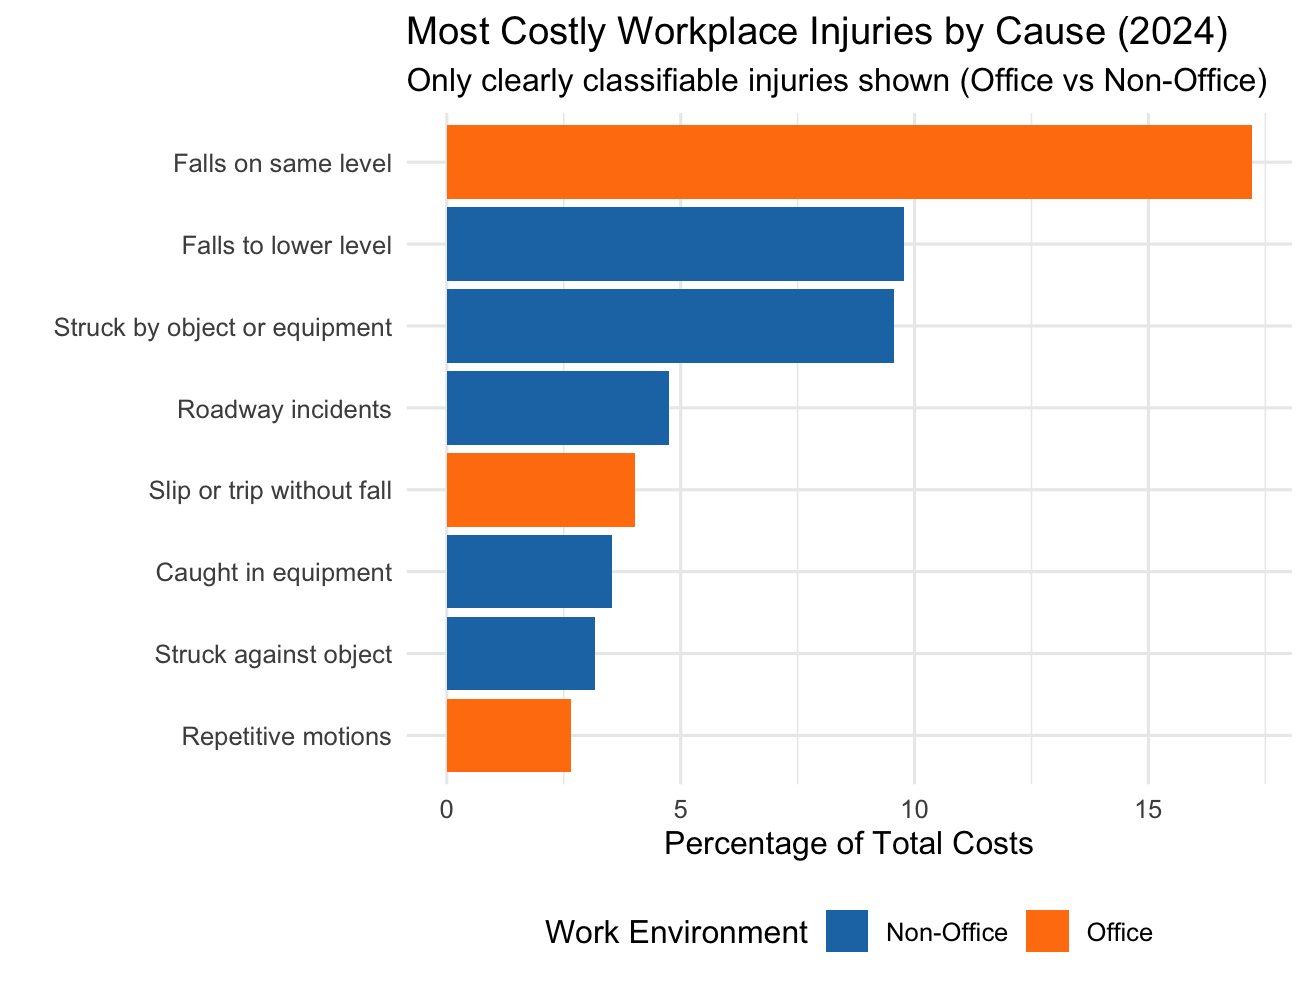
\includegraphics[width=5.72917in,height=\textheight,keepaspectratio]{officecomparison.png}

}

\caption{Figure 1 highlights that office-related falls contribute more
than twice the costs of non-office falls (21.2\% vs.~9.8\%).}

\end{figure}%

\begin{longtable}[]{@{}lrl@{}}
\caption{Table 1: Breakdown of Injury Costs by Cause and Work
Environment.}\tabularnewline
\toprule\noalign{}
Injury Cause & \% of Costs & Environment \\
\midrule\noalign{}
\endfirsthead
\toprule\noalign{}
Injury Cause & \% of Costs & Environment \\
\midrule\noalign{}
\endhead
\bottomrule\noalign{}
\endlastfoot
Falls on same level & 17.21 & Office \\
Falls to lower level & 9.78 & Non-Office \\
Struck by object or equipment & 9.56 & Non-Office \\
Roadway incidents & 4.76 & Non-Office \\
Slip or trip without fall & 4.02 & Office \\
Caught in equipment & 3.54 & Non-Office \\
Struck against object & 3.17 & Non-Office \\
Repetitive motions & 2.65 & Office \\
\end{longtable}

Falls represent a major cost driver in both settings, but office falls
(same level + slips) account for 21.2\% of fall-related costs, compared
to 9.8\% for non-office falls. This highlights the financial burden of
seemingly minor but frequent office accidents.

\begin{longtable}[]{@{}lrr@{}}
\caption{Table 2: Fall-Related Injury Costs by Work
Environment}\tabularnewline
\toprule\noalign{}
Environment & Total \% of Costs & Proportion of Falls \\
\midrule\noalign{}
\endfirsthead
\toprule\noalign{}
Environment & Total \% of Costs & Proportion of Falls \\
\midrule\noalign{}
\endhead
\bottomrule\noalign{}
\endlastfoot
Non-Office & 9.78 & 32\% \\
Office & 21.23 & 68\% \\
\end{longtable}

\section{Regional Workplace Injury
Trends}\label{regional-workplace-injury-trends}

\begin{figure}[H]

{\centering 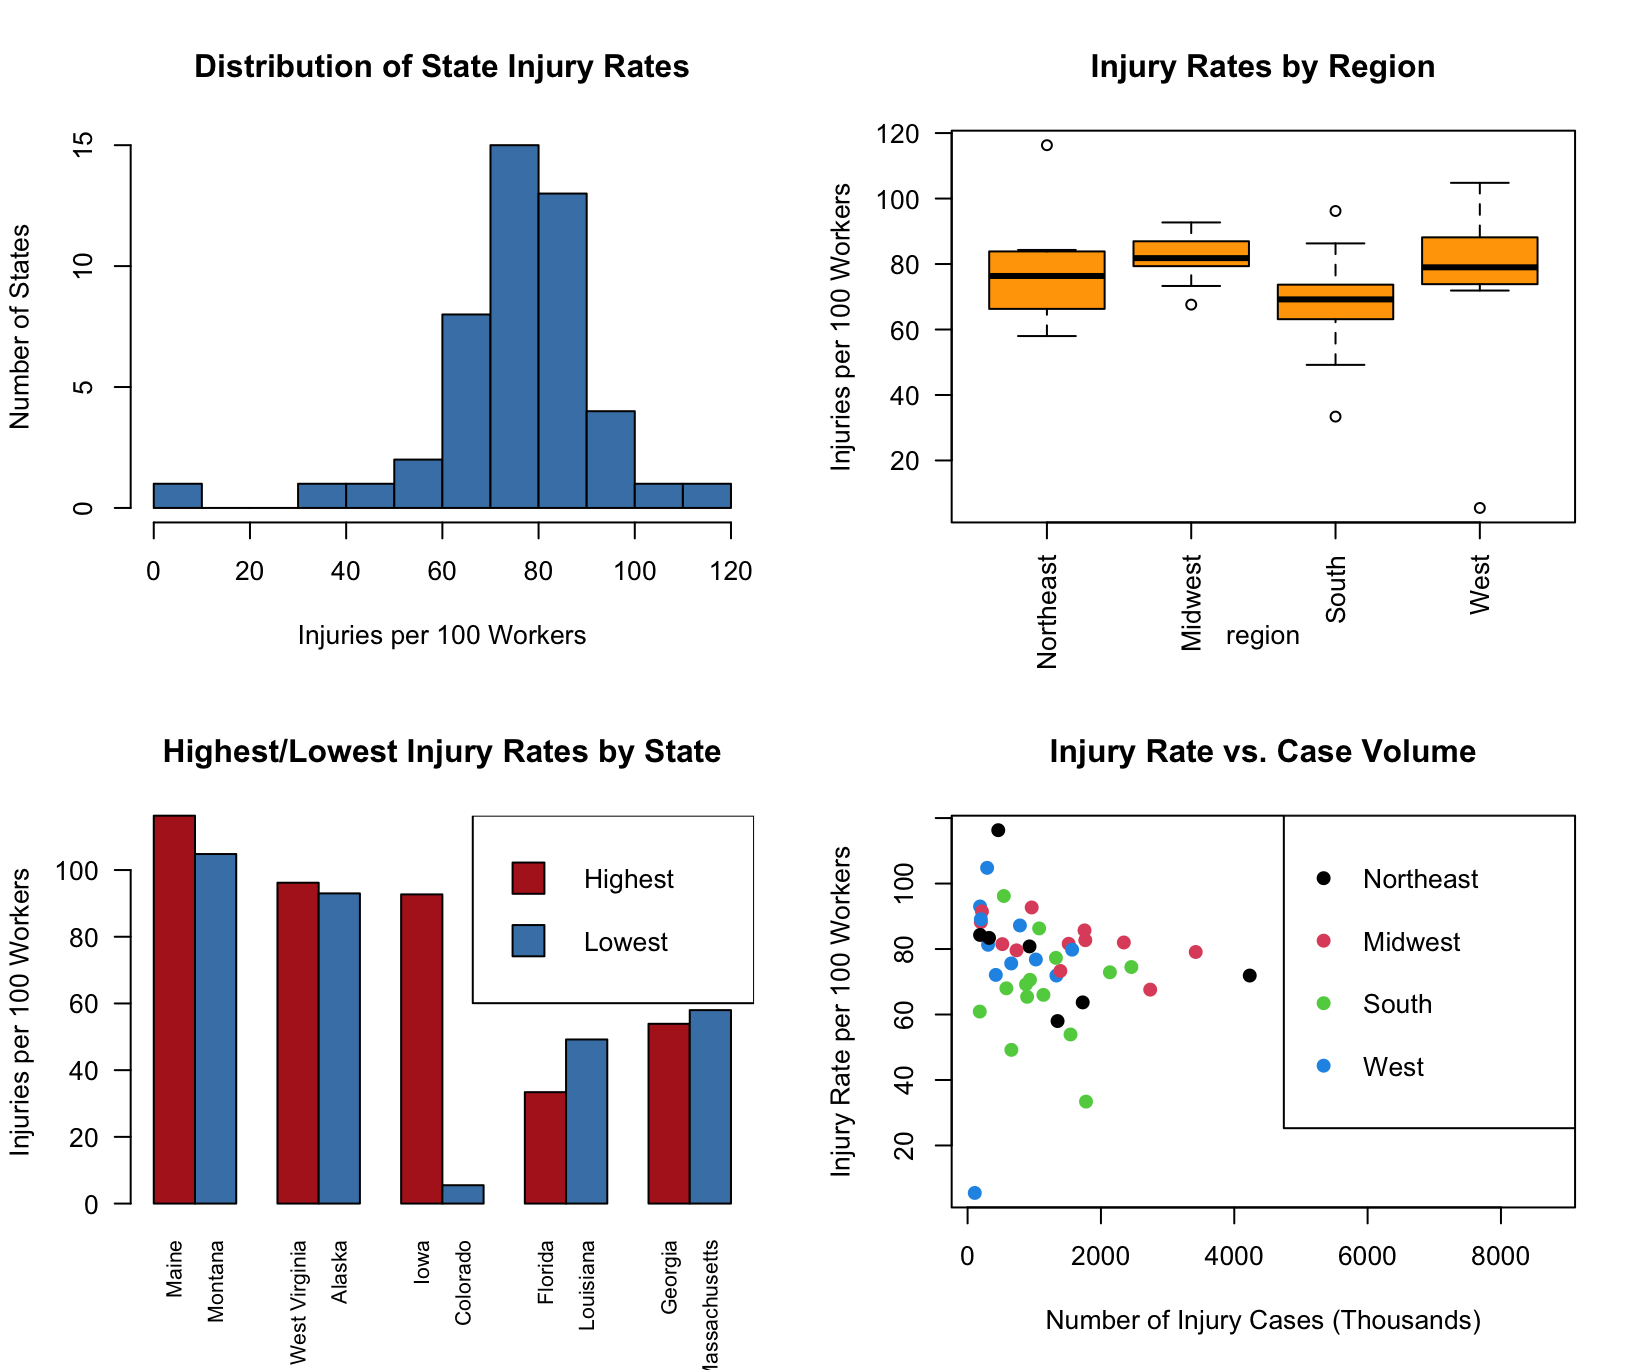
\includegraphics[width=5.72917in,height=\textheight,keepaspectratio]{statecompare.png}

}

\caption{Figure 2 shows the Midwest has both the highest median and most
variable injury rates.}

\end{figure}%

\begin{longtable}[]{@{}
  >{\raggedright\arraybackslash}p{(\linewidth - 8\tabcolsep) * \real{0.1310}}
  >{\raggedleft\arraybackslash}p{(\linewidth - 8\tabcolsep) * \real{0.1667}}
  >{\raggedleft\arraybackslash}p{(\linewidth - 8\tabcolsep) * \real{0.1548}}
  >{\raggedleft\arraybackslash}p{(\linewidth - 8\tabcolsep) * \real{0.2143}}
  >{\raggedleft\arraybackslash}p{(\linewidth - 8\tabcolsep) * \real{0.3333}}@{}}
\caption{Table 3: Workplace Injury Rates by Region}\tabularnewline
\toprule\noalign{}
\begin{minipage}[b]{\linewidth}\raggedright
Region
\end{minipage} & \begin{minipage}[b]{\linewidth}\raggedleft
Average Rate
\end{minipage} & \begin{minipage}[b]{\linewidth}\raggedleft
Median Rate
\end{minipage} & \begin{minipage}[b]{\linewidth}\raggedleft
Number of States
\end{minipage} & \begin{minipage}[b]{\linewidth}\raggedleft
Total Injuries (Thousands)
\end{minipage} \\
\midrule\noalign{}
\endfirsthead
\toprule\noalign{}
\begin{minipage}[b]{\linewidth}\raggedright
Region
\end{minipage} & \begin{minipage}[b]{\linewidth}\raggedleft
Average Rate
\end{minipage} & \begin{minipage}[b]{\linewidth}\raggedleft
Median Rate
\end{minipage} & \begin{minipage}[b]{\linewidth}\raggedleft
Number of States
\end{minipage} & \begin{minipage}[b]{\linewidth}\raggedleft
Total Injuries (Thousands)
\end{minipage} \\
\midrule\noalign{}
\endhead
\bottomrule\noalign{}
\endlastfoot
Midwest & 82.1 & 81.8 & 12 & 17559.2 \\
Northeast & 78.4 & 76.3 & 8 & 14637.4 \\
West & 76.3 & 79.0 & 12 & 15210.3 \\
South & 67.6 & 69.2 & 15 & 24878.8 \\
\end{longtable}

On the state level, Maine (116.3 per 100 workers) has the highest injury
rate, over 20 times greater than Colorado (5.5 per 100 workers), which
has the lowest. However, correlation analysis (r = -0.09, p = 0.553)
indicates no significant relationship between case volume and injury
rate, suggesting that higher total injury counts do not necessarily
translate to higher rates at the state level.

\begin{longtable}[]{@{}
  >{\raggedright\arraybackslash}p{(\linewidth - 8\tabcolsep) * \real{0.1343}}
  >{\raggedright\arraybackslash}p{(\linewidth - 8\tabcolsep) * \real{0.2239}}
  >{\raggedleft\arraybackslash}p{(\linewidth - 8\tabcolsep) * \real{0.1940}}
  >{\raggedleft\arraybackslash}p{(\linewidth - 8\tabcolsep) * \real{0.2836}}
  >{\raggedright\arraybackslash}p{(\linewidth - 8\tabcolsep) * \real{0.1642}}@{}}
\caption{Table 4: States with the Highest and Lowest Workplace Injury
Rates}\tabularnewline
\toprule\noalign{}
\begin{minipage}[b]{\linewidth}\raggedright
Rank
\end{minipage} & \begin{minipage}[b]{\linewidth}\raggedright
State
\end{minipage} & \begin{minipage}[b]{\linewidth}\raggedleft
Injury Rate
\end{minipage} & \begin{minipage}[b]{\linewidth}\raggedleft
Cases (Thousands)
\end{minipage} & \begin{minipage}[b]{\linewidth}\raggedright
Region
\end{minipage} \\
\midrule\noalign{}
\endfirsthead
\toprule\noalign{}
\begin{minipage}[b]{\linewidth}\raggedright
Rank
\end{minipage} & \begin{minipage}[b]{\linewidth}\raggedright
State
\end{minipage} & \begin{minipage}[b]{\linewidth}\raggedleft
Injury Rate
\end{minipage} & \begin{minipage}[b]{\linewidth}\raggedleft
Cases (Thousands)
\end{minipage} & \begin{minipage}[b]{\linewidth}\raggedright
Region
\end{minipage} \\
\midrule\noalign{}
\endhead
\bottomrule\noalign{}
\endlastfoot
Lowest & Massachusetts & 58.0 & 1349.6 & Northeast \\
Lowest & Georgia & 53.9 & 1543.7 & South \\
Lowest & Louisiana & 49.2 & 656.3 & South \\
Lowest & Florida & 33.4 & 1776.2 & South \\
Lowest & Colorado & 5.5 & 107.5 & West \\
Highest & Maine & 116.3 & 459.8 & Northeast \\
Highest & Montana & 104.8 & 292.8 & West \\
Highest & West Virginia & 96.2 & 543.2 & South \\
Highest & Alaska & 93.0 & 186.9 & West \\
Highest & Iowa & 92.7 & 961.2 & Midwest \\
\end{longtable}

\chapter{Draft: Intro/Conclusions}\label{draft-introconclusions}

\chapter{Introduction}\label{introduction-1}

In 2023, Amazon was fined \$7,000 by OSHA following the death of a
warehouse worker linked to unsafe conditions
((\textbf{StaffFortWayneAmazon?})). The company also faced a \$60,000
penalty for exposing employees to additional hazards
((\textbf{PalmerAmazonCitedLabor?})), and has been the subject of over
50 OSHA investigations since 2020, with fines totaling more than \$6
million ({``Amazon {Is Fined Nearly} \$6 {Million Over Warehouse Work
Quotas} - {The New York Times}''} (n.d.)). These incidents emphasize the
real costs of workplace injuries, where employers face not only human
tragedy but also legal liability and reputational damage. Nationally,
U.S. businesses lose an estimated \$167 billion annually due to
workplace injuries ({``Work {Injury Costs}''} (n.d.)).

While industrial settings often dominate safety conversations, office
environments are frequently overlooked, despite accounting for 23.9\% of
preventable injury costs. This report explores whether office workers
face greater injury risks than non-office workers, particularly in terms
of injury frequency and cost. Using Bureau of Labor Statistics (BLS)
data, I analyzed injury trends across workplace types and regions,
identifying the most costly injury types, and examining where injury
rates are highest.

Findings revealed that while non-office settings have higher overall
injury rates, office environments experience a disproportionate share of
same-level falls, responsible for 17.2\% of total injury costs. These
results suggest that companies should reallocate safety resources toward
office settings, possibly reducing liability exposure and overall costs
despite common assumptions that non-office settings are riskier.

\chapter{Conclusion}\label{conclusion}

This analysis examined injury costs and risks in both office and
non-office environments, as well as regional variations in injury rates.
The findings show that office environments account for 23.9\% of injury
costs, while non-office environments contribute 30.8\%. Falls are the
leading cause of injury in both environments, with office settings
bearing a disproportionate share of fall-related costs at 21.2\%,
compared to 9.8\% in non-office environments. Although regional injury
rates varied, ANOVA results indicated no statistically significant
differences. Maine had the highest injury rate, while Colorado had the
lowest. Additionally, the correlation analysis showed no meaningful
relationship between injury volume and injury rate.

While informative, this study has limitations, primarily due to the
scope and limitations of publicly available data. The dataset may not
fully capture unreported incidents, variations in workplace practices
across industries, or inconsistencies in data collection. Future
research could assess the effectiveness of safety policies, the quality
of their implementation, and other factors influencing injury rates.
Expanding the dataset to include more variables and detailed industry
breakdowns would offer a more comprehensive understanding of injury
risks.

\section{Recommendations}\label{recommendations}

Based on the findings, I recommend the following:

\begin{itemize}
\item
  \textbf{Fall Prevention in Office Settings:} Given the high proportion
  of fall-related costs in office environments, companies should invest
  in targeted fall prevention programs. These could include routine
  maintenance of flooring and employee education around slip and trip
  hazards.
\item
  \textbf{Region-Specific Safety Assessments:} Despite the lack of
  statistically significant regional differences, variation still exists
  at the state level. Businesses should consider conducting local
  assessments to tailor safety interventions to the specific risks and
  needs of each region.
\end{itemize}

\chapter{Draft: Executive Summary}\label{draft-executive-summary}




\end{document}
